\section{Detectors for High Energy Physics}
\label{sec:detectors}

In this section we review the basic concepts that drive the design of the LHC detectors, including ATLAS.

\subsection{Identification of Particles}

The ability to accurately identify particles and reconstruct their energy is what drives the design of detectors for high energy physics. In a detector, different sub-systems are able to capture different types of particle interaction, and the combination of the information collected by each of them allows to identify particles (or at least assign them to families, such as neutral or charged hadrons). A typical schema of the subdetectors sequence is shown in Fig. \ref{fig:detector:interaction}. The innermost layer, closer to the interaction point, is the \textit{tracking system}, dedicated to the measurement of the signed change and momentum of charged particles. The following layers are the electromagnetic and hadronic \textit{calorimeters}, that measure the energy of particles with electromagnetic and hadronic interactions respectively. The outermost layer is dedicated to the \textit{muon system}: because of their large mass (about 200 times more than electrons) muons do not produce electromagnetic showers and are therefore easy to identify as they are the only particles that reach the external part of the detector.

\begin{figure}[ht]
\centering
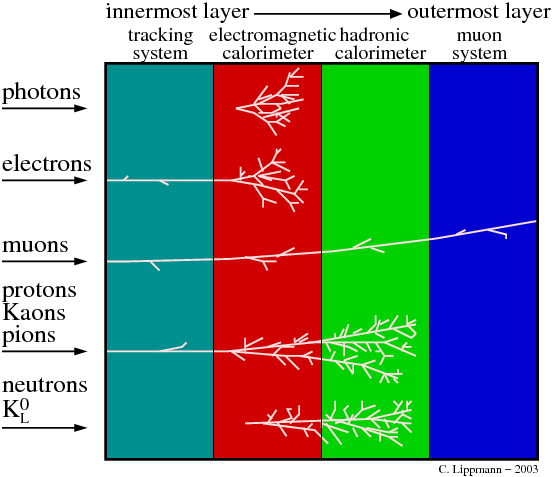
\includegraphics[width=0.6\textwidth]{figures/detector/particles_in_detector}
\caption{Components of a typical detector for physics at colliders. Different particles are identified by the distinctive signatures in the subdetectors. Figure from Ref. \cite{Lippmann:2011bb}.}
\label{fig:detector:interaction}
\end{figure}


\subsection{Tracking and Spectrometry}
\label{sec:dec:tracking}
A tracking device measures the traces left by charged particles passing through it. To allow the determination of the momentum and the charge of a particle, a tracking device needs to be accompanied by a magnetic field. 

The relative uncertainty on the momentum is given by:
\begin{equation}
\frac{\sigma_p}{p} = \frac{p}{0.3 B L^2}\sigma \sqrt{C_N}
\end{equation}


\subsection{Calorimetry}
\label{sec:dec:calo}

Calorimeters can measure the energy of both charged and neutral particles through a destructive measurement: the energy of the particles is deposited in the detector material and transformed into a measurable quantity. Because of their sensitivity to a wide variety of particles, good energy resolution and relatively small size, they are very attractive devices for accelerator physics experiments \cite{RevModPhys.75.1243} \cite{Wigmans:2000vf}.

When the incident particle interacts with the material of the calorimeter it develops a cascade of particles (\textit{shower}), with different characteristics for electromagnetic and hadronic interactions, described in the next two sections. Different types of calorimeters are necessary to capture the two typologies. The energy of the shower is decreased by the interactions happening in the \textit{absorber} material, while the \textit{active} material provides the conversion of the energy in a charge or light signal. In \textit{sampling calorimeters} layers of absorber and active material are alternated in sequence, while in \textit{homogeneous calorimeters} a single material carries out both functions.


\subsubsection{Electromagnetic Cascade}

The type of interaction that electromagnetically-interacting particles have with the detector depends on their energy. The average fractional energy loss in lead for electrons and positrons and the photon interaction cross section in lead are shown in Fig. \ref{fig:det:shower_elec} (a) and (b) respectively. 

\begin{figure}[ht]
\centering
\subfigure{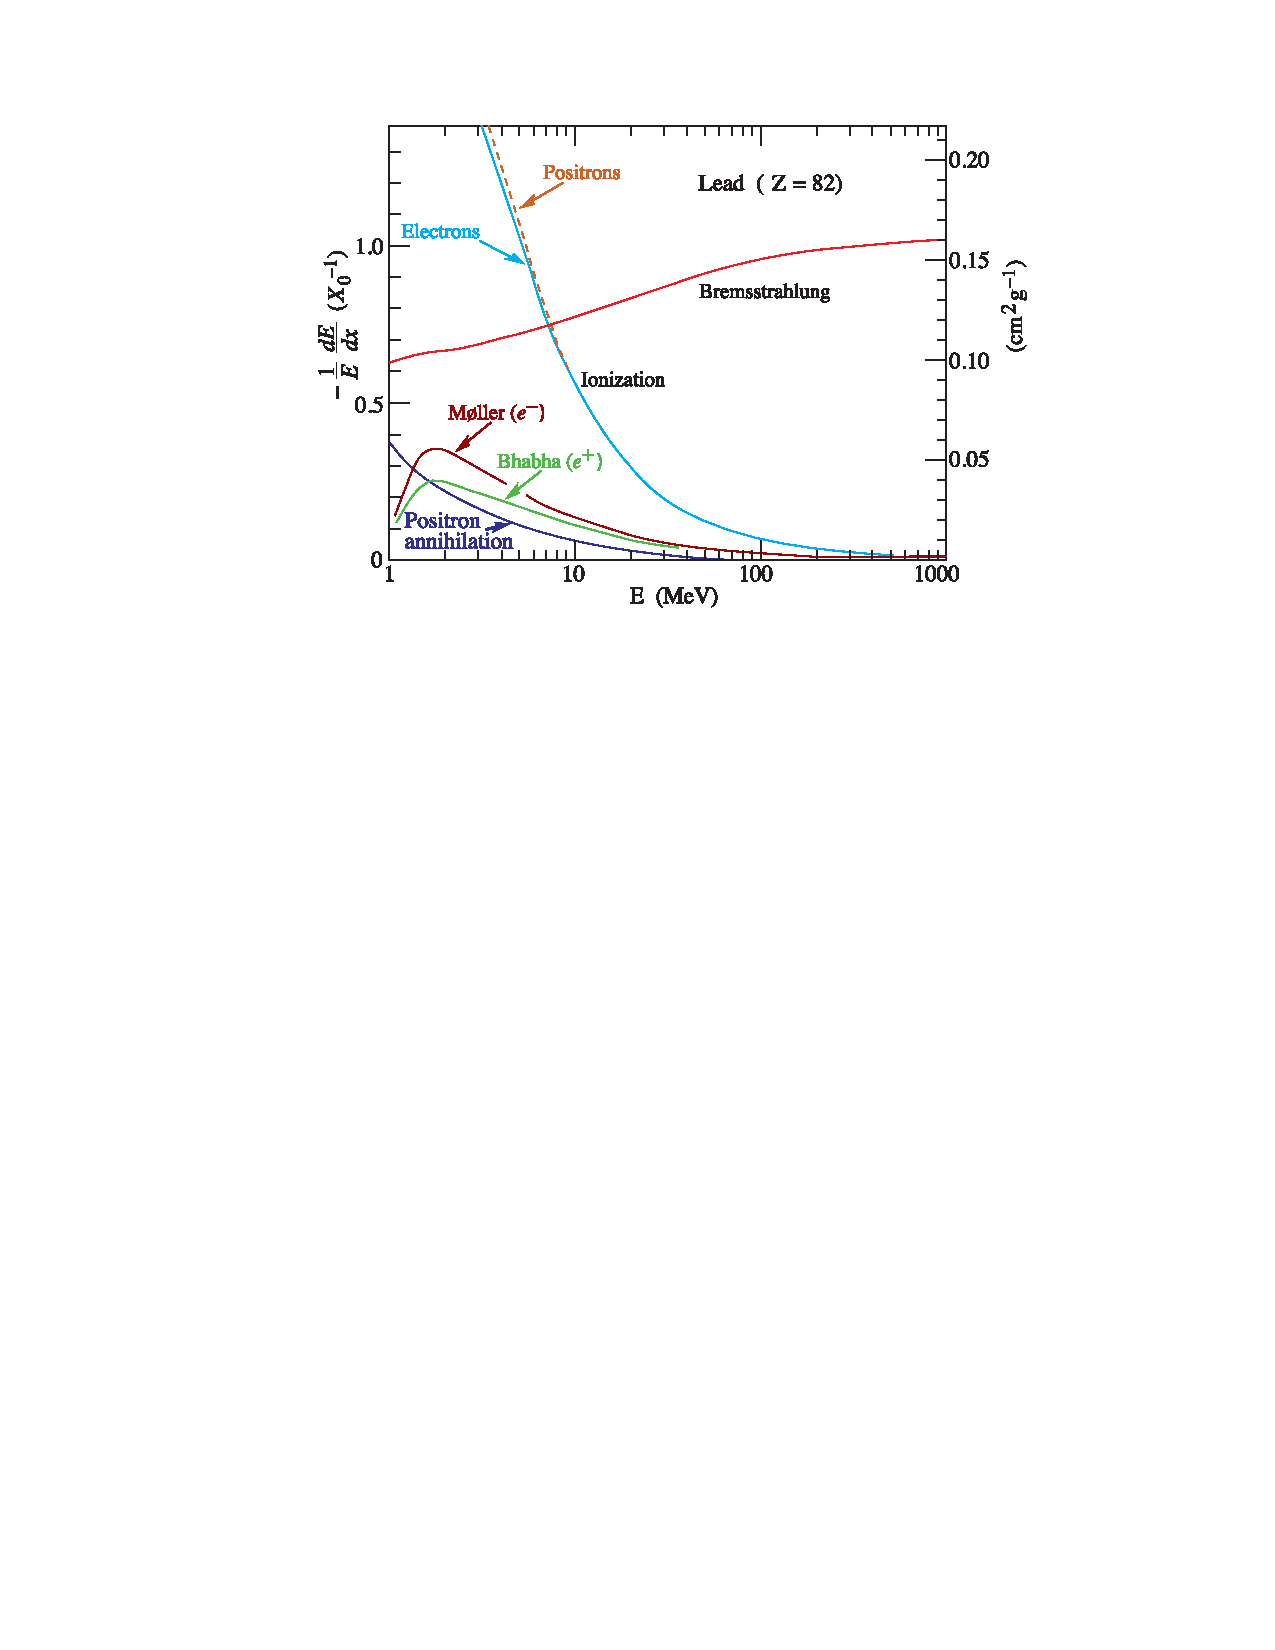
\includegraphics[width=0.58\textwidth]{figures/detector/electron_energy_loss}}
\subfigure{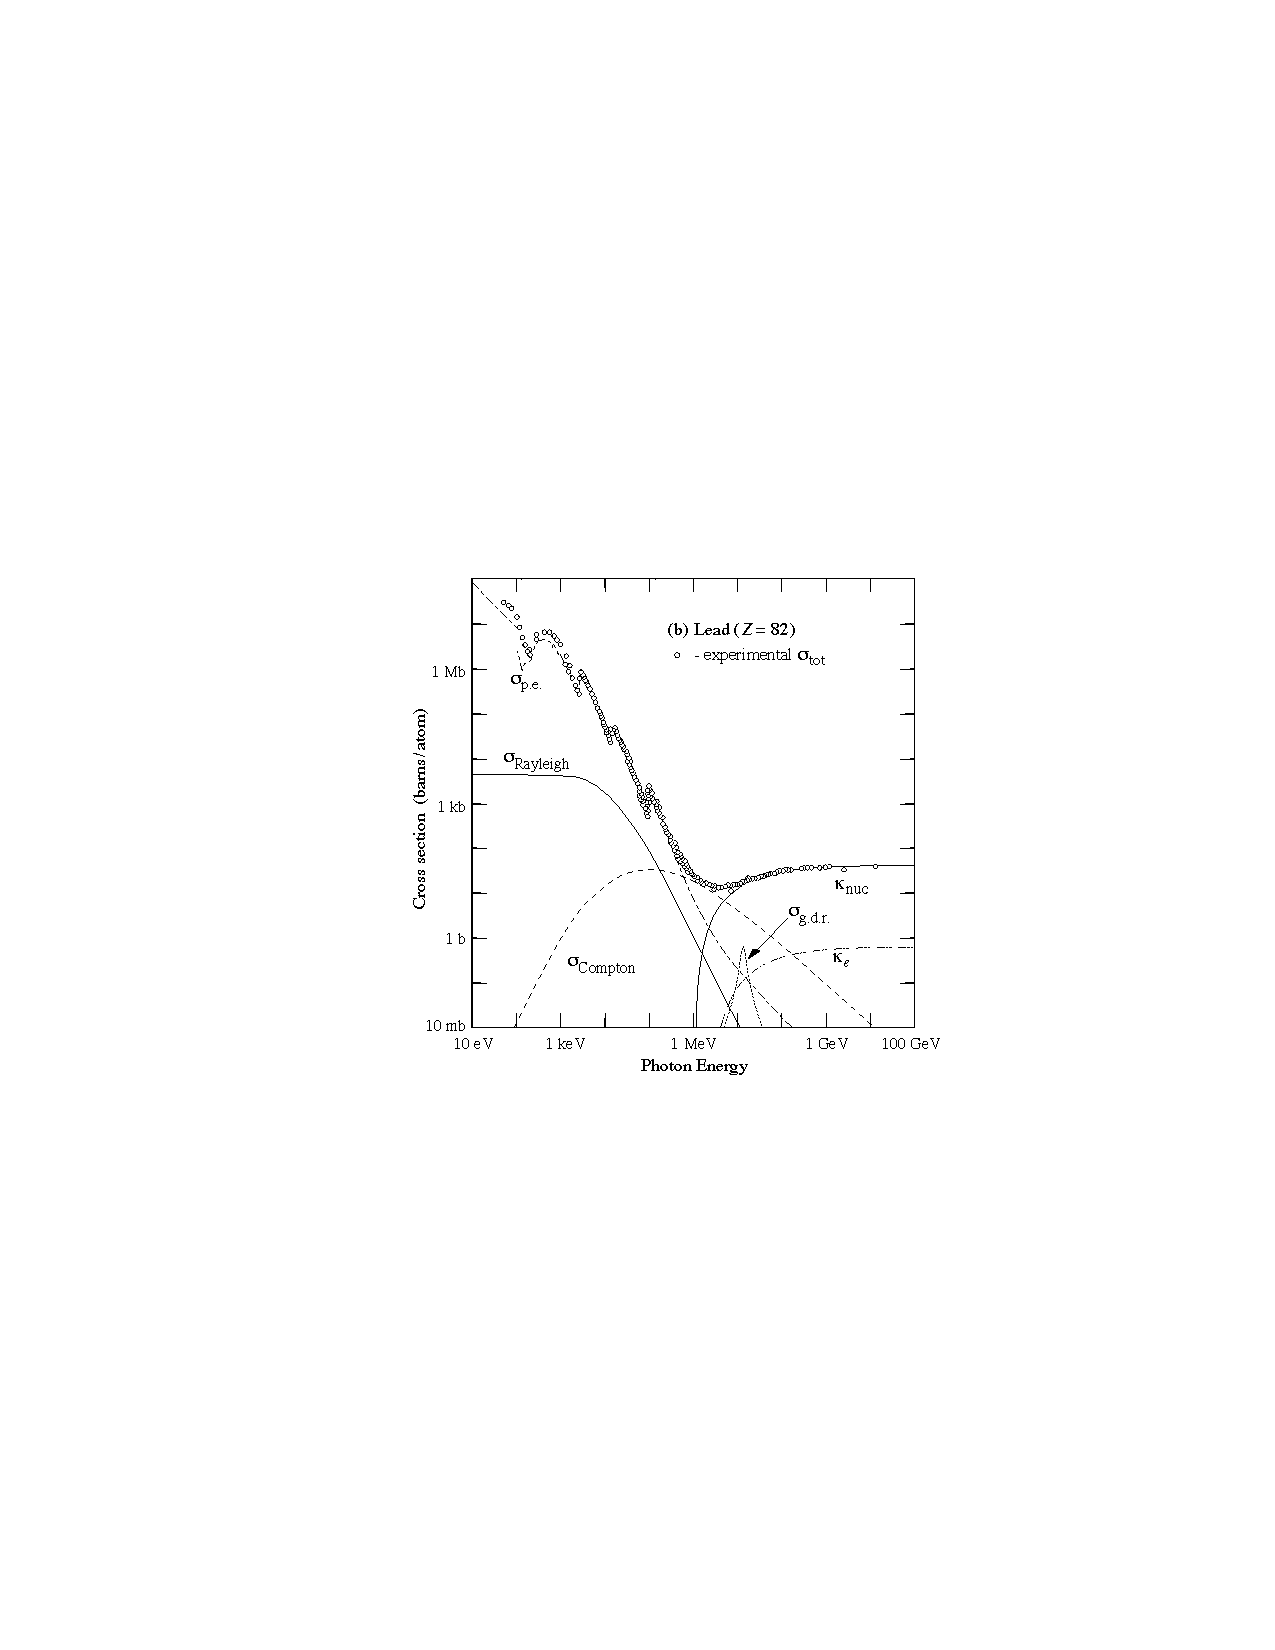
\includegraphics[width=0.4\textwidth]{figures/detector/photon_xsec}}
\caption{(a) Fractional energy loss per radiation length in lead as a function of the electron (positron) energy. (b) Photon interaction cross section in lead. Figures from Ref. \cite{Patrignani:2016xqp}. }
\label{fig:det:shower_elec}
\end{figure}


When electrons, positrons and photons with energies above 1 GeV traverse a block of material the produce a cascade of particles (\textit{electromagnetic shower}): electrons and positrons can emit a photon by Bremsstrahlung, and a photon (thanks to the interaction with a nucleus) can turn into an electron-positron pair (pair production is indicated with the symbol $\kappa_{nucl}$ in Fig. \ref{fig:det:shower_elec} (b)). A schematic view of the evolution of an electromagnetic shower is shown  in Fig. \ref{fig:det:shower_elec}(a). 

\begin{figure}[ht]
\centering
\subfigure{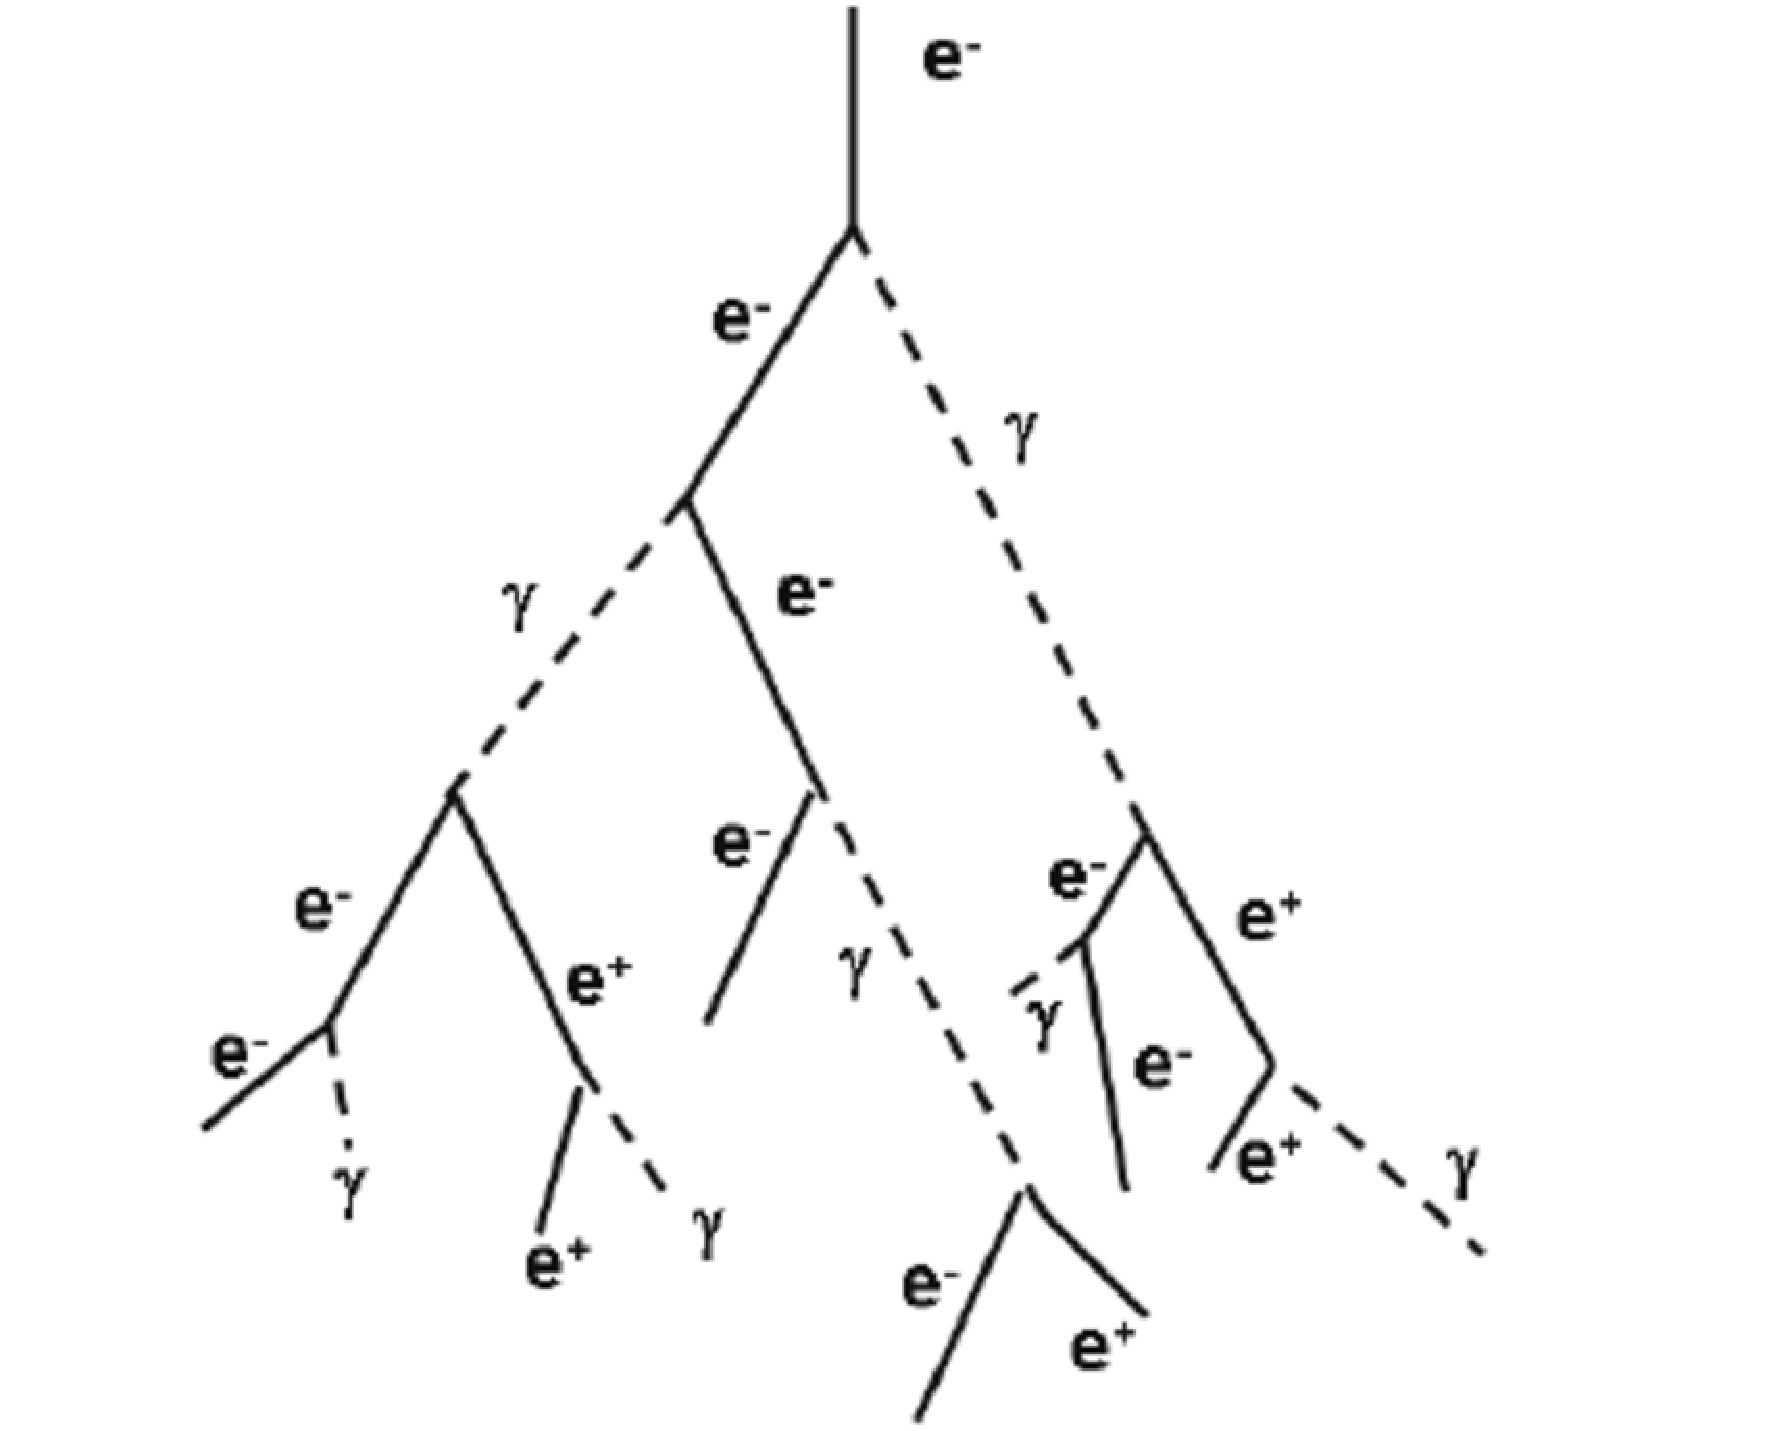
\includegraphics[width=0.45\textwidth]{figures/detector/elec_shower}}
\subfigure{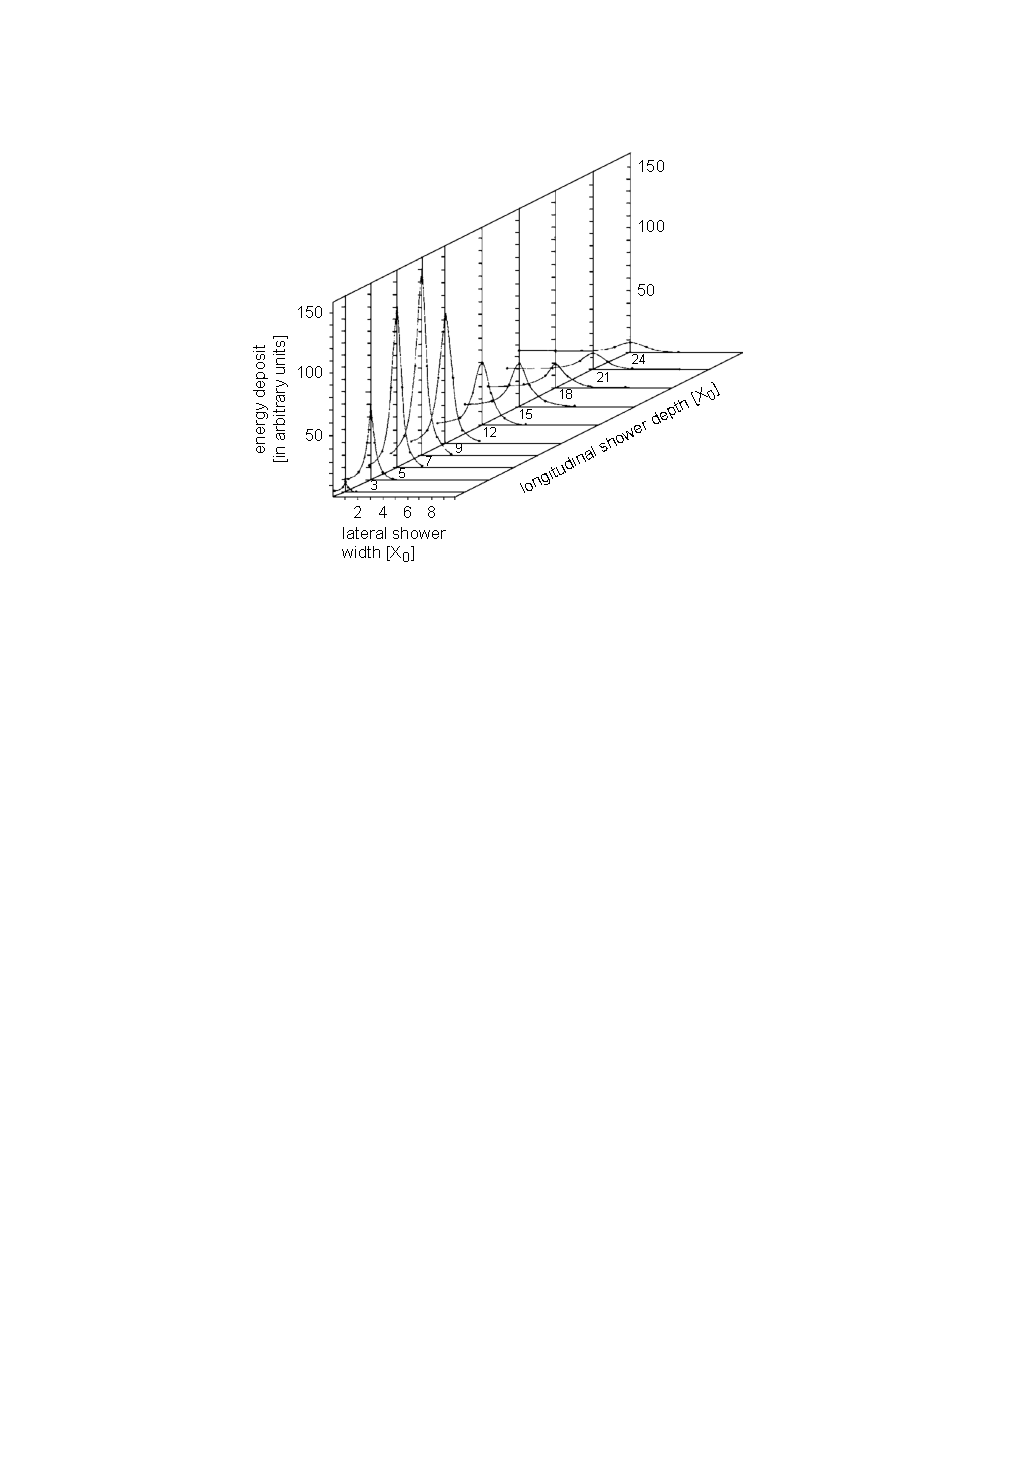
\includegraphics[width=0.52\textwidth]{figures/detector/elec_shower_lateral}}
\caption{(a) Sketch of the evolution of an electromagnetic shower. (b) Lateral and longitudianl evolution of the shower form 6-GeV electons. Figure from Ref. \cite{grupen_shwartz_2008}.}
\label{fig:det:shower_elec}
\end{figure}


The main parameter to describe the evolution of an electromagnetic shower is the \textit{radiation length} ($X_0$), defined as the distance over which an electron reduces its energy to $\frac{1}{e}$ of the initial value, and corresponds also to $\frac{7}{9}$ of the mean free path for pair production for a photon. The radiation length depends on the characteristics of the material:
\begin{equation}
X_0 [\frac{g}{cm^2}] = \frac{716 \frac{g}{ cm^2} A }{Z(Z+1) \ln\left(287/\sqrt{Z}\right)} \; ,
\end{equation}

where $A$ and $Z$ are the atomic and mass number of the material. If we define $t = \frac{x}{X_0}$ as the shower depth relative to the radiation length, the maximum number of produced particles occurs at:
\begin{equation}
t_{max} = \frac{\ln \left(E_0/E_c\right)}{ln\left(2\right)} \;,
\end{equation}
and 25 radiation lengths contain about 99\% of the total shower energy. The typical values for the interaction length are of the order of the $cm$ (e.g. 0.56 cm for lead, 1.76 cm for iron \cite{Patrignani:2016xqp}), allowing for electromagnetic calorimeters of compact dimensions. 
The lateral with of the shower, determined mainly by multiple scattering, increases with depth and is defined in terms of the Moli\'ere radius:
\begin{equation}
R_M = \frac{21 MeV \; X_0[\frac{g}{cm^2}]}{E_c [MeV]} \; .
\end{equation}
A cylinder of radius 2$R_M$ contains about 95\% of the shower; for most calorimeters $R_M$ has a value of few centimeters, so electromagnetic showers are quite narrow. The longitudinal and lateral development of the shower induced in lead by 6-GeV electrons is shown in Fig. \ref{fig:det:shower_elec}(b).

Once the electrons in the shower have an energy lower than the \textit{critical energy} ($E_c$, defined as the energy where the loss through Bremsstrahlung equals the one through ionization), the shower stops as the energy is dissipated mostly through ionization for electrons and photoelectric effect for photons, and not anymore through the creation of new particles.


We have noticed in section \ref{sec:dec:tracking} how the resolution of the momentum measurement in a magnetic spectrometer decreases with the increase of the momentum itself. Instead, the relative energy resolution in a calorimeter improves for high-energy particles, and can be written in the parametric form:

\begin{equation}
\frac{\sigma_E}{E} = \sqrt{\left(\frac{a}{\sqrt{E}} \right)^2 + \left( \frac{b}{E} \right)^2 + c^2 } \; .
\end{equation}

The first term of the sum in quadrature reflects the \textit{stochastic} nature of the shower development: ignoring the instrumental effects, the energy resolution of a calorimeter is proportional to the square root of the total track length, which is in turn proportional to the initial energy. The contribution of this term is small in homogeneous calorimeters, while is larger in sampling calorimeters (because of fluctuations of the fraction of energy deposited in the absorber) and it grows with the thickness of the absorber layers; typical values for $a$ are 5-20\% if the energy is expressed in GeV. The second term is the \textit{noise term} coming from the electronic noise of the readout chain; this term is in general more relevant for calorimeters producing charge signals than for those producing light signals, and can become the dominant term for particles with energy below one GeV. The last term is a constant deriving from instrumental effects that produce a non-uniform detector response, including for example energy lost outside the detector volume and radiation damage; this becomes the dominant term at high energies and is typically $<1\%$. 



\subsubsection{Hadronic Shower}

The difference between electromagnetic calorimeters and hadronic calorimeters finds its origin in the more complicated nature of strong interactions compared to the electromagnetic ones.

A sketch of the evolution of an hadronic shower is shown in Fig. \ref{fig:det:shower_had}(a)

Fig. \ref{fig:det:shower_had}(b) shows the lateral shower profile for 10-GeV pions in iron.

\begin{figure}[ht]
\centering
\subfigure{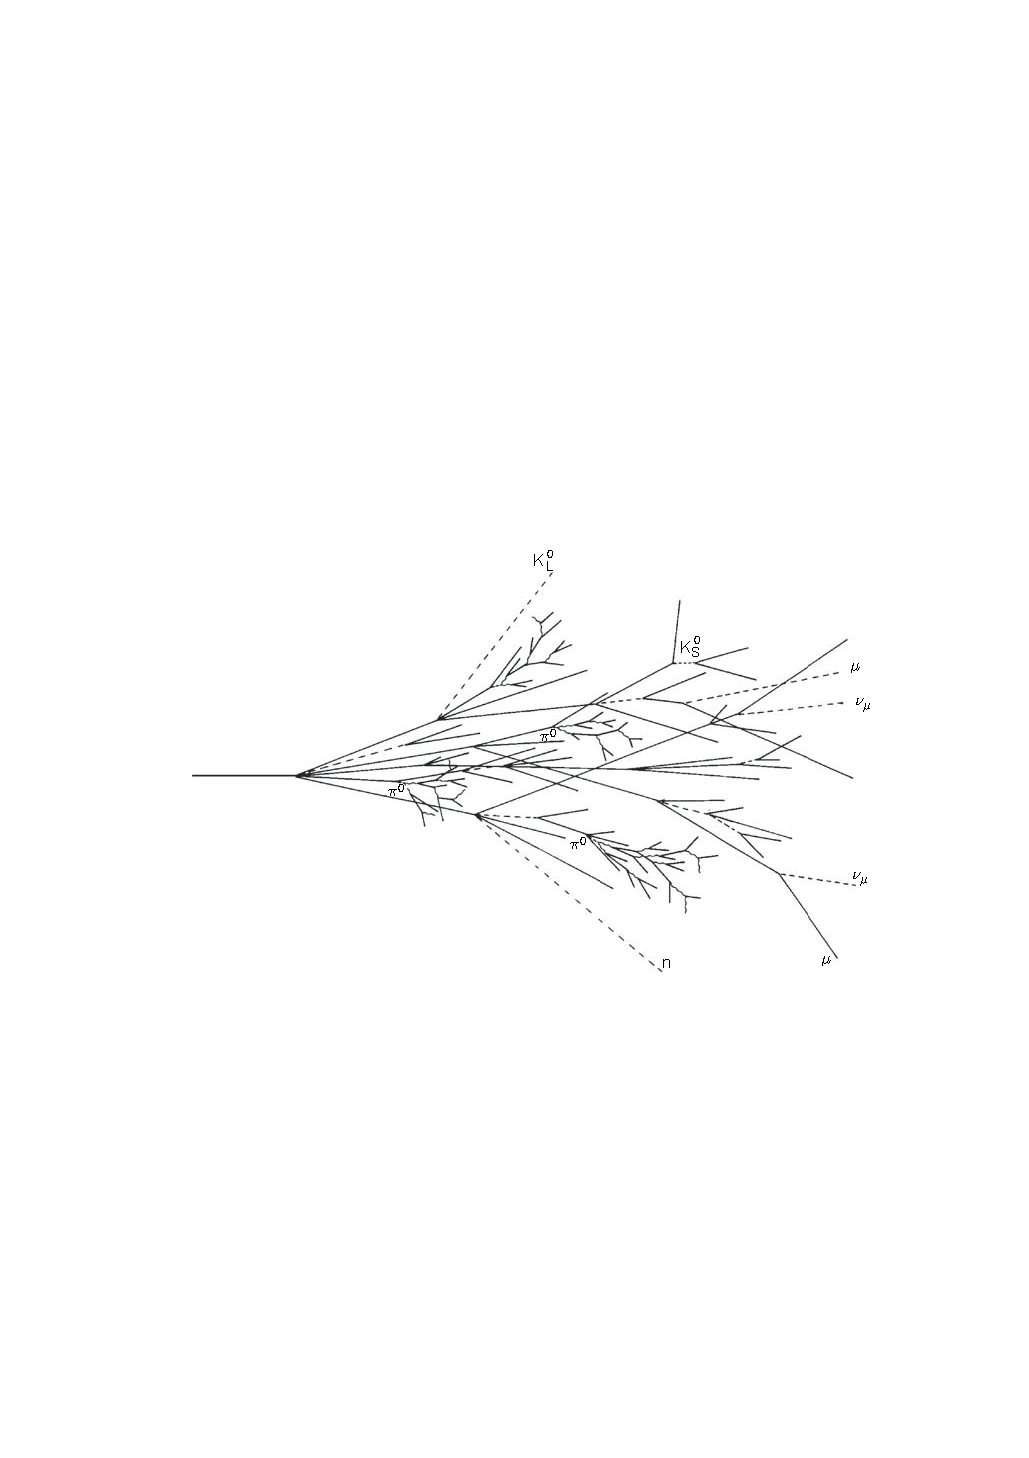
\includegraphics[width=0.48\textwidth]{figures/detector/hadron_shower}}
\subfigure{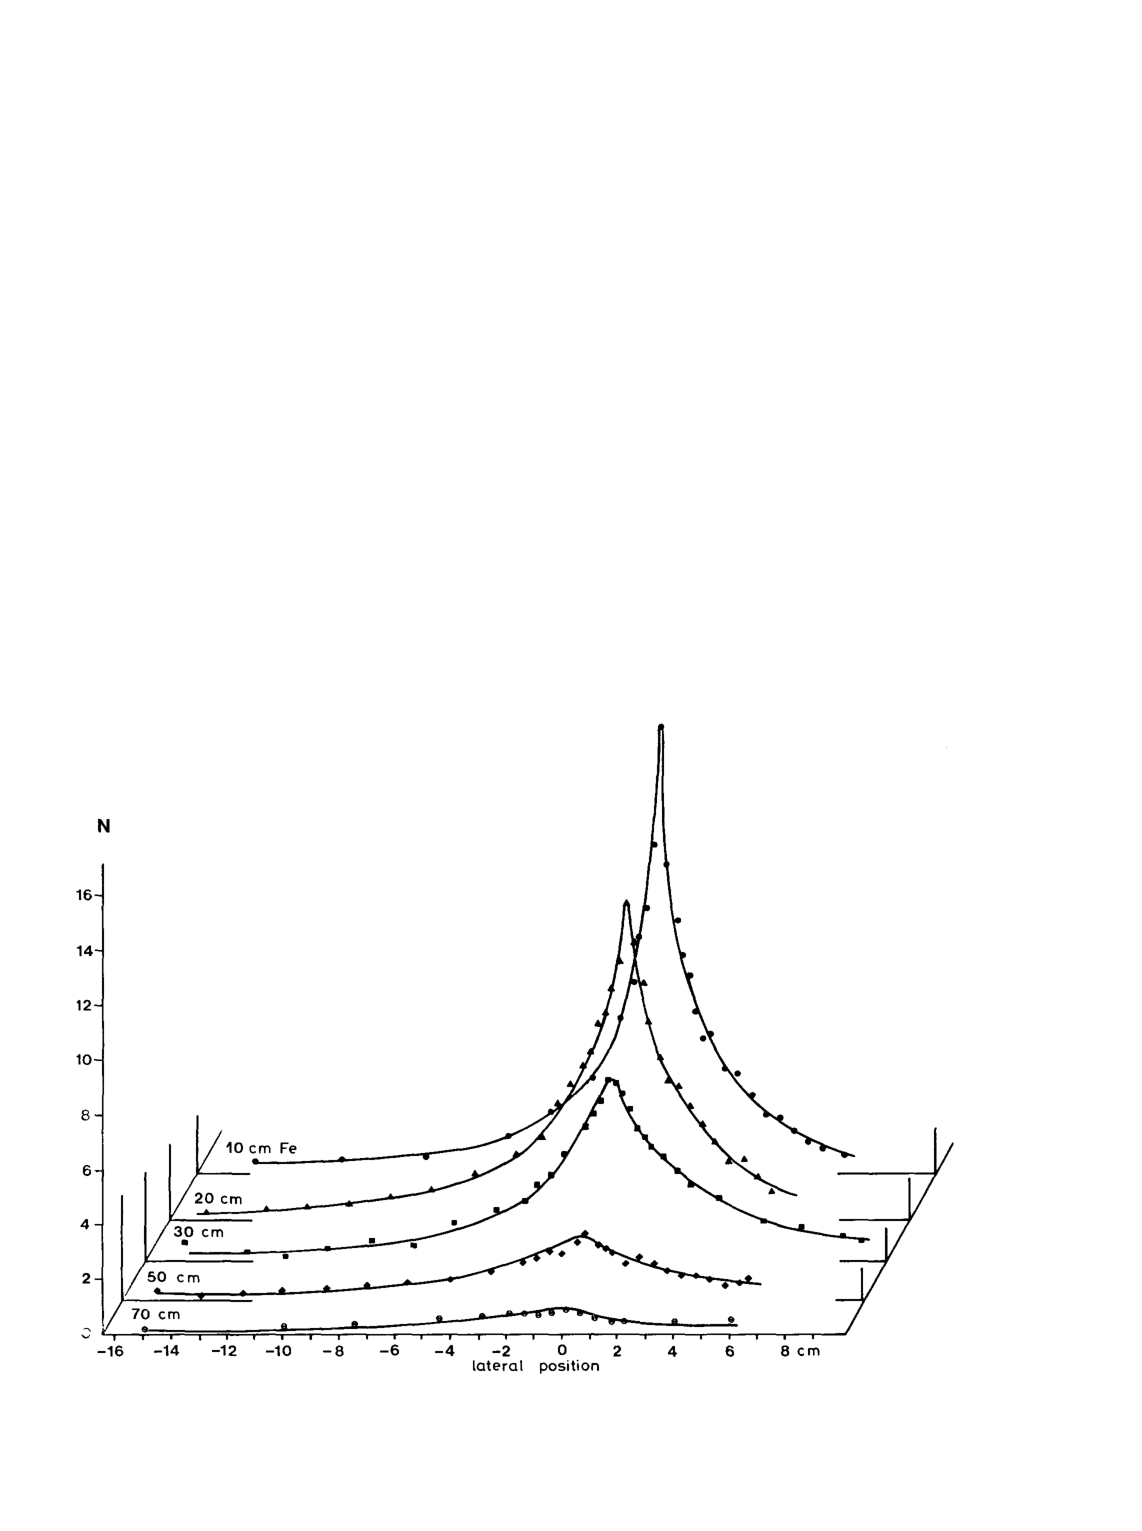
\includegraphics[width=0.48\textwidth]{figures/detector/hadron_shower_lateral}}
\caption{(a) Sketch of the evolution of an hadronic shower. Figure from Ref. \cite{grupen_shwartz_2008}. (b) Lateral energy distribution of shower induced by 10-GeV $\pi^-$, measured at a depth of 10, 20, 30, 50 and 70 cm in Fe. Fig from Ref. \cite{FRIEND1976505}.}
\label{fig:det:shower_had}
\end{figure}

